% Provenance (never printed): see sources/outline_sources.md (Year 2: field and laboratory methods ---
% igneous and metamorphic petrography, chemical analysis by XRF, ICP-MS and microprobe, isotope mass
% spectrometry, a mapping campaign). Modelled on Book 3 ch. 6.
% Textures: BGS RR 99-02 (Robertson 1999), Open University Virtual Microscope, Carleton BH250,
% UCSB Geology 102C (Hacker); QAPF: BGS RR 99-06 (Gillespie and Styles 1999); instruments: SERC
% Geochemical Instrumentation and Analysis sheets (EPMA, WDS, XRF, TIMS, MC-ICPMS); XRF procedure
% and reference-material results: USGS OFR 02-223 and its chapter T (Taggart and Siems 2002); Sr
% isotopes: CIAAW; spike and mass bias: Cheong, Jeong and Kwon (2014). Ledger rows in
% sources/ledger/book4.md; curves and stations from figdata/bachelor-2/labmethods.py, numbers from
% the Book 4 second-writer scratch calculator calc/ch31.py. Observation only: the professional work
% is described in the third person.
\chapter{Métodos de campo e de laboratório II}\label{ch:b2:field-lab-methods-2}

Cada número dos capítulos de petrologia deste livro começou como uma rocha num saco, uma lâmina delgada sob um
microscópio e um pó num instrumento. Uma composição mineral lançada num diagrama de fases, o
teor de sílica que dá nome a uma lava, a razão isotópica do estrôncio que rastreia uma fonte mantélica: cada um
saiu de uma cadeia de operações que começou num afloramento, e cada um carrega os erros de cada
elo. Este capítulo segue essa cadeia para as rochas do embasamento das Varden Hills: ler as texturas
em lâmina delgada, contar os minerais, analisar a rocha total, depois os minerais isolados, depois os isótopos,
perguntando a cada passo quão bom é o número.

\begin{recall}
\textbf{Do volume do primeiro ano}: a estação de campo, a caderneta de campo, a amostra orientada, a lâmina delgada,
o microscópio de polarização, a luz plano-polarizada, os polarizadores cruzados; a identificação óptica dos minerais
formadores de rocha; o recálculo de uma fórmula mineral a partir de uma análise de óxidos sobre um número fixo de oxigênios,
e do ferro férrico pelo balanço de cargas; a foliação e a xistosidade; a isócrona, a razão inicial e a
reta de mínimos quadrados. \textbf{Dos livros de química}: a espectrometria de massa, o plasma indutivamente acoplado;
a curva de calibração, o limite de detecção, o limite de quantificação, a precisão, a veracidade, o viés,
a repetibilidade, o desvio-padrão da média. \textbf{Dos livros de física}: os raios X característicos
e a lei de Moseley; a lei de Bragg; a tensão superficial; a propagação de incertezas.
\textbf{Dos livros de matemática}: a distribuição binomial, sua média e sua variância.
\textbf{Do \cref{ch:b2:magmatic-series}}: a \omterm{def:b2:magmatic-series:qapf}{composição modal}, o \omterm{def:b2:magmatic-series:qapf}{diagrama QAPF}.
\textbf{Do \cref{ch:b2:isotope-geochemistry}}: o \omterm{def:b2:isotope-geochemistry:tracer}{traçador isotópico radiogênico}, o \omterm{def:b2:isotope-geochemistry:standards}{padrão isotópico de referência}.
\end{recall}

\section{Petrografia: as texturas como uma história}\label{sec:b2:field-lab-methods-2:petrography}

O volume do primeiro ano usou o microscópio de polarização para identificar minerais. Um petrógrafo também lê
como os grãos estão arranjados, porque o arranjo registra a ordem em que cresceram. Duas
texturas são as testemunhas mais comuns da cristalização a partir de um líquido magmático e da recristalização no
estado sólido.

\begin{definition}[Textura ofítica, textura granoblástica]\label{def:b2:field-lab-methods-2:textures}
Uma rocha ígnea tem \emph{textura ofítica}\index{textura ofítica} quando grandes cristais de piroxênio
englobam pequenas ripas de plagioclásio orientadas ao acaso; a textura é típica do diabásio, do gabro
e do basalto. Uma rocha metamórfica tem \emph{textura granoblástica}\index{textura granoblástica} quando
é um agregado de cristais aproximadamente equidimensionais e de tamanho semelhante, em muitos casos anédricos,
cujos limites retos se encontram três a três em ângulos próximos de \ang{120}.
\end{definition}
% ledger: carletonB:ophitic, ouVM:textures, bgsM:textures

Numa rocha ofítica as ripas englobadas são inteiras e euédricas, e o piroxênio preenche o espaço
entre elas: o plagioclásio cresceu primeiro, o piroxênio em volta dele. Os ângulos de \ang{120} de uma
\omterm{def:b2:field-lab-methods-2:textures}{textura granoblástica} são os de grãos que tiveram tempo de ajustar seus limites; o material didático de petrografia lê essas junções
tríplices como sinal de equilíbrio químico e textural. O ângulo decorre de um equilíbrio de forças, os limites de grão puxando sua
linha comum como películas de sabão (a tensão superficial, dos livros de física).
% ledger: ouVM:equilibrium

\begin{proposition}[Ângulos numa junção tríplice]\label{prop:b2:field-lab-methods-2:triple}
Suponha-se que três limites de grão se encontrem ao longo de uma linha, com tensões (energias por unidade de área) $\gamma_1$,
$\gamma_2$, $\gamma_3$, e seja $\theta_i$ o ângulo entre os dois limites que não o
limite $i$. No equilíbrio,
\begin{equation}
\frac{\gamma_1}{\sin\theta_1} = \frac{\gamma_2}{\sin\theta_2} = \frac{\gamma_3}{\sin\theta_3},
\label{eq:b2:field-lab-methods-2:lami}
\end{equation}
e três tensões iguais encontram-se em três ângulos de \ang{120}.
\end{proposition}

\begin{proof}
Num plano perpendicular à junção, cada limite puxa a junção ao longo de seu próprio traço
com a força $\gamma_i$ por unidade de comprimento. No equilíbrio as três forças somam zero, de modo que, colocadas
uma após a outra, elas fecham um triângulo. O ângulo do triângulo oposto ao lado $\gamma_i$ é
$\pi - \theta_i$, cujo seno é $\sin\theta_i$, e a lei dos senos no triângulo dá
\eqref{eq:b2:field-lab-methods-2:lami}. Se as três tensões são iguais, o triângulo é
equilátero, e cada ângulo externo $\theta_i$ vale $\pi - \pi/3 = 2\pi/3$, isto é, \ang{120}.
\end{proof}

\begin{omfigure}
\centering
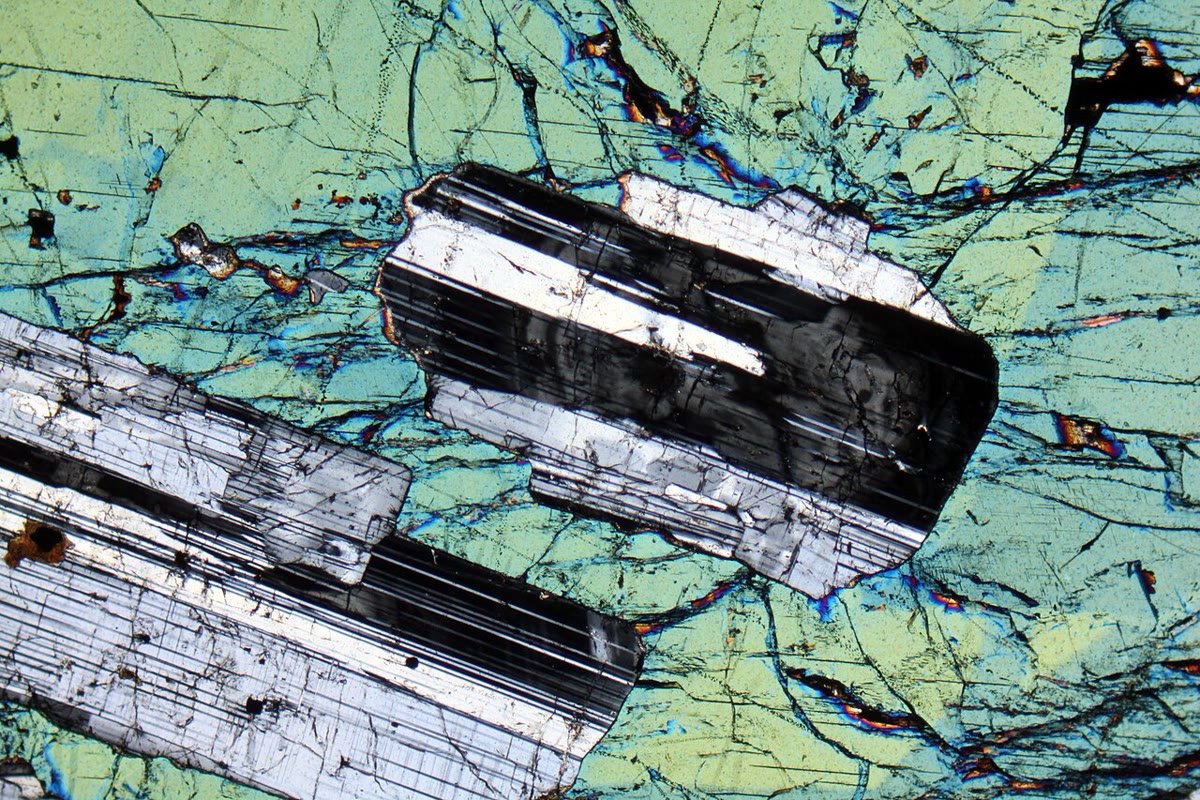
\includegraphics[height=4.6cm]{images/book4/b2-31-ophitic.jpg}\quad
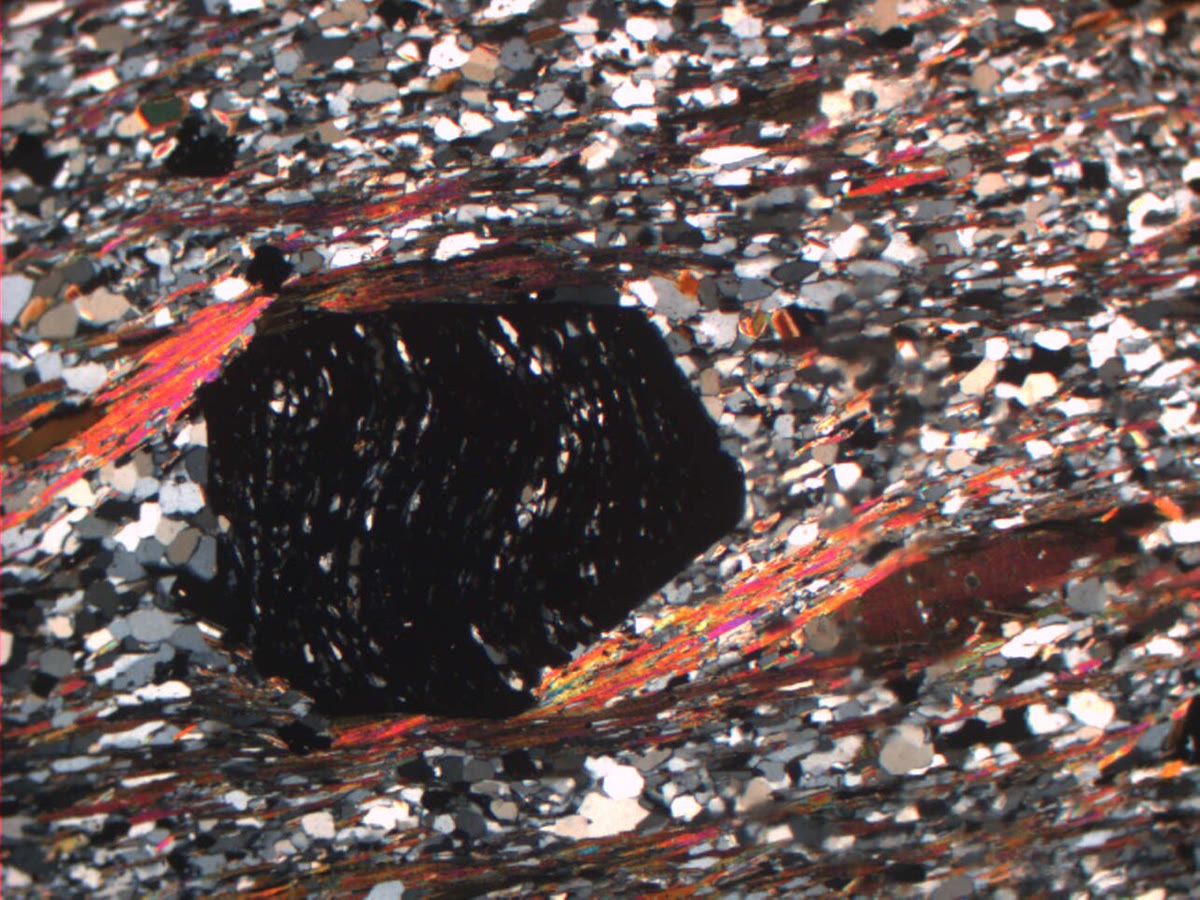
\includegraphics[height=4.6cm]{images/book4/b2-31-garnet-porphyroblast.jpg}
\par\smallskip{\small Duas texturas entre polarizadores cruzados. À esquerda: um único cristal de augita (azul
e verde) engloba ripas de plagioclásio listradas por sua geminação, o arranjo de uma \omterm{def:b2:field-lab-methods-2:textures}{textura
ofítica}; campo de visão de \qty{7}{mm}. Fotografia de Strekeisen, CC BY-SA 4.0 (Wikimedia Commons).
À direita: um granada--mica xisto. A granada, preta porque é isótropa, é um grande cristal que
cresceu no estado sólido; inclusões de quartzo a atravessam em trilhas, e a foliação de muscovita
(cores vivas), biotita (marrom) e quartzo (cinza) contorna-a. Fotografia de Jackdann88,
CC BY 3.0 (Wikimedia Commons).}
\end{omfigure}
% ledger: photo:b2-31-ophitic, photo:b2-31-garnet

Os minerais metamórficos não crescem todos no mesmo ritmo. Algumas espécies crescem sobre as outras em cristais muito grandes,
que englobam os pequenos grãos à sua volta à medida que crescem.

\begin{definition}[Porfiroblasto, poiquiloblasto, trilha de inclusões, coroa]\label{def:b2:field-lab-methods-2:porphyroblast}
Um \emph{porfiroblasto}\index{porfiroblasto} é um grande cristal que cresceu durante o \omterm{def:b2:metamorphic-facies:metamorphism}{metamorfismo}
numa matriz de granulação mais fina; granada, estaurolita, cordierita e cloritoide formam-nos, de
milímetros a vários centímetros de diâmetro. Um \emph{poiquiloblasto}\index{poiquiloblasto} é um
porfiroblasto que contém muitas inclusões de outros minerais. Uma \emph{trilha de
inclusões}\index{trilha de inclusões} é uma linha de inclusões alinhadas dentro de um porfiroblasto, que
preserva a trama da matriz no momento em que o cristal cresceu sobre ela. Uma
\emph{coroa}\index{coroa (textura de reação)} é uma orla de um ou mais minerais novos que envolve completamente
um mineral que estava se decompondo, porque deixara de ser estável com seus
vizinhos: uma textura de reação, congelada antes que a reação se completasse.
\end{definition}
% ledger: bgsM:textures, ouVM:textures

Comparar a \omterm{def:b2:field-lab-methods-2:porphyroblast}{trilha de inclusões} ($S_i$, a trama interna) com a foliação fora do cristal
($S_e$, a trama externa) data o crescimento de um \omterm{def:b2:field-lab-methods-2:porphyroblast}{porfiroblasto} em relação à deformação que
produziu a foliação. Os critérios abaixo, desenhados na figura, são os das notas didáticas correntes.
% ledger: ucsbH:inclusion-trails

\begin{method}[Datar um porfiroblasto por suas trilhas de inclusões]\label{met:b2:field-lab-methods-2:timing}
Encontre uma seção cortada perpendicularmente à foliação e compare $S_i$ e $S_e$.
\begin{enumerate}
  \item \textbf{Inclusões ao acaso}, $S_e$ defletida em volta do cristal: ele cresceu antes da formação da
        foliação (\emph{pré-tectônico}).
  \item \textbf{$S_i$ reta truncada na borda}, descontínua com uma $S_e$ defletida: ele cresceu
        sobre uma foliação mais antiga, entre duas deformações (\emph{intertectônico}).
  \item \textbf{$S_i$ curva}, contínua com $S_e$: ele cresceu enquanto a foliação se formava, girando
        ou sendo sobrecrescido à medida que crescia (\emph{sintectônico}; a espiral de uma granada em bola de neve).
  \item \textbf{$S_i$ reta contínua com uma $S_e$ não defletida}: ele cresceu depois da foliação
        (\emph{pós-tectônico}).
\end{enumerate}
\end{method}

\begin{omfigure}
\centering
\begin{tikzpicture}[x=1cm, y=1cm, font=\scriptsize]
% schematic after the criteria of ledger ucsbH:inclusion-trails
% panel 1: pre-tectonic
\begin{scope}[shift={(0,0)}]
\draw[omExo, line width=0.5pt] (-1.5,0.95) .. controls (-0.6,0.95) and (-0.5,0.85) .. (0,0.85) .. controls (0.5,0.85) and (0.6,0.95) .. (1.5,0.95);
\draw[omExo, line width=0.5pt] (-1.5,-0.95) .. controls (-0.6,-0.95) and (-0.5,-0.85) .. (0,-0.85) .. controls (0.5,-0.85) and (0.6,-0.95) .. (1.5,-0.95);
\draw[omExo, line width=0.5pt] (-1.5,0.45) .. controls (-0.9,0.45) and (-0.85,0.78) .. (0,0.78) .. controls (0.85,0.78) and (0.9,0.45) .. (1.5,0.45);
\draw[omExo, line width=0.5pt] (-1.5,-0.45) .. controls (-0.9,-0.45) and (-0.85,-0.78) .. (0,-0.78) .. controls (0.85,-0.78) and (0.9,-0.45) .. (1.5,-0.45);
\draw[omExo, line width=0.5pt] (-1.5,0) -- (-0.78,0); \draw[omExo, line width=0.5pt] (0.78,0) -- (1.5,0);
\filldraw[fill=omThm!15, draw=omThm, line width=0.6pt] (0,0) circle (0.72);
\draw[black, line width=0.7pt] (-0.4,0.2) -- (-0.25,0.35); \draw[black, line width=0.7pt] (0.1,0.35) -- (0.3,0.2);
\draw[black, line width=0.7pt] (-0.35,-0.2) -- (-0.15,-0.25); \draw[black, line width=0.7pt] (0.2,-0.15) -- (0.25,-0.4);
\draw[black, line width=0.7pt] (-0.05,0.05) -- (0.05,-0.1); \draw[black, line width=0.7pt] (0.35,0.0) -- (0.5,0.12);
\node at (0,-1.3) {pré-tectônico};
\end{scope}
% panel 2: inter-tectonic
\begin{scope}[shift={(3.4,0)}]
\draw[omExo, line width=0.5pt] (-1.5,0.95) .. controls (-0.6,0.95) and (-0.5,0.85) .. (0,0.85) .. controls (0.5,0.85) and (0.6,0.95) .. (1.5,0.95);
\draw[omExo, line width=0.5pt] (-1.5,-0.95) .. controls (-0.6,-0.95) and (-0.5,-0.85) .. (0,-0.85) .. controls (0.5,-0.85) and (0.6,-0.95) .. (1.5,-0.95);
\draw[omExo, line width=0.5pt] (-1.5,0.45) .. controls (-0.9,0.45) and (-0.85,0.78) .. (0,0.78) .. controls (0.85,0.78) and (0.9,0.45) .. (1.5,0.45);
\draw[omExo, line width=0.5pt] (-1.5,-0.45) .. controls (-0.9,-0.45) and (-0.85,-0.78) .. (0,-0.78) .. controls (0.85,-0.78) and (0.9,-0.45) .. (1.5,-0.45);
\draw[omExo, line width=0.5pt] (-1.5,0) -- (-0.78,0); \draw[omExo, line width=0.5pt] (0.78,0) -- (1.5,0);
\filldraw[fill=omThm!15, draw=omThm, line width=0.6pt] (0,0) circle (0.72);
\begin{scope}
\clip (0,0) circle (0.66);
\foreach \k in {-0.6,-0.3,0,0.3,0.6} {\draw[black, line width=0.7pt, dash pattern=on 2pt off 1.5pt] (-0.8,\k-0.45) -- (0.8,\k+0.45);}
\end{scope}
\node at (0,-1.3) {intertectônico};
\end{scope}
% panel 3: syn-tectonic
\begin{scope}[shift={(6.8,0)}]
\draw[omExo, line width=0.5pt] (-1.5,0.8) -- (1.5,0.8);
\draw[omExo, line width=0.5pt] (-1.5,-0.8) -- (1.5,-0.8);
\draw[omExo, line width=0.5pt] (-1.5,0.4) -- (-0.6,0.4); \draw[omExo, line width=0.5pt] (0.6,0.4) -- (1.5,0.4);
\draw[omExo, line width=0.5pt] (-1.5,0) -- (-0.72,0); \draw[omExo, line width=0.5pt] (0.72,0) -- (1.5,0);
\draw[omExo, line width=0.5pt] (-1.5,-0.4) -- (-0.6,-0.4); \draw[omExo, line width=0.5pt] (0.6,-0.4) -- (1.5,-0.4);
\filldraw[fill=omThm!15, draw=omThm, line width=0.6pt] (0,0) circle (0.72);
\draw[black, line width=0.7pt, dash pattern=on 2pt off 1.5pt] (-0.6,0.4) .. controls (-0.35,0.4) and (-0.2,0.3) .. (-0.05,0.4) .. controls (0.1,0.5) and (0.35,0.4) .. (0.6,0.4);
\draw[black, line width=0.7pt, dash pattern=on 2pt off 1.5pt] (-0.72,0) .. controls (-0.3,0) and (-0.3,-0.45) .. (0,0) .. controls (0.3,0.45) and (0.3,0) .. (0.72,0);
\draw[black, line width=0.7pt, dash pattern=on 2pt off 1.5pt] (-0.6,-0.4) .. controls (-0.35,-0.4) and (-0.1,-0.5) .. (0.05,-0.4) .. controls (0.2,-0.3) and (0.35,-0.4) .. (0.6,-0.4);
\node at (0,-1.3) {sintectônico};
\end{scope}
% panel 4: post-tectonic
\begin{scope}[shift={(10.2,0)}]
\foreach \k in {-0.8,-0.4,0,0.4,0.8} {\draw[omExo, line width=0.5pt] (-1.5,\k) -- (1.5,\k);}
\filldraw[fill=omThm!15, draw=omThm, line width=0.6pt] (0,0) circle (0.72);
\begin{scope}
\clip (0,0) circle (0.66);
\foreach \k in {-0.8,-0.4,0,0.4,0.8} {\draw[black, line width=0.7pt, dash pattern=on 2pt off 1.5pt] (-0.8,\k) -- (0.8,\k);}
\end{scope}
\node at (0,-1.3) {pós-tectônico};
\end{scope}
\end{tikzpicture}
\par\smallskip{\small \omterm{def:b2:field-lab-methods-2:porphyroblast}{Trilhas de inclusões} (em preto, tracejadas) num \omterm{def:b2:field-lab-methods-2:porphyroblast}{porfiroblasto} (vermelho) e a foliação
fora dele (cinza), em seções perpendiculares à foliação (esquemático). Da esquerda para a direita:
inclusões crescidas antes da foliação, que se curva em volta do cristal; uma trama mais antiga reta truncada
na borda; uma trilha que se curva até a foliação, tendo o cristal girado enquanto crescia; uma
trilha reta que prolonga a foliação não perturbada.}
\end{omfigure}

A petrografia também é quantitativa. As proporções dos minerais de uma rocha ígnea de granulação grossa
dão-lhe nome no \omterm{def:b2:magmatic-series:qapf}{diagrama QAPF} (\cref{ch:b2:magmatic-series}), e são medidas ao
microscópio.

\begin{definition}[Análise modal, contagem de pontos]\label{def:b2:field-lab-methods-2:modal}
Uma \emph{análise modal}\index{análise modal} é a medida da \omterm{def:b2:magmatic-series:qapf}{composição modal} de uma
rocha. Na \emph{contagem de pontos}\index{contagem de pontos}, uma lâmina
delgada é deslocada sob os fios do retículo do microscópio em passos iguais ao longo de uma malha regular, e
o mineral sob os fios do retículo é registrado em cada ponto; a proporção dos pontos que
caem sobre um mineral estima sua proporção na rocha.
\end{definition}

\begin{proposition}[O que a contagem de pontos mede, e com que qualidade]\label{prop:b2:field-lab-methods-2:counting}
(a) Numa rocha sem orientação preferencial, a fração de área de um mineral numa seção posicionada
ao acaso tem, em média, o valor de sua fração volumétrica. (b) Se $n$ pontos caem independentemente
sobre um mineral de fração de área $p$, a proporção contada $\hat p = k/n$ tem média $p$ e
desvio-padrão
\begin{equation}
\sigma = \sqrt{\frac{p(1-p)}{n}} , \qquad\text{de modo que}\qquad n = \frac{p(1-p)}{\sigma^2}
\label{eq:b2:field-lab-methods-2:binomial}
\end{equation}
pontos são necessários para atingir um desvio-padrão $\sigma$.
\end{proposition}

\begin{proof}
(a) Corte-se um bloco de rocha de altura $H$ em seções paralelas de área $S$. O volume do
mineral é $\int_0^H a(z)\,\mathrm{d}z$, onde $a(z)$ é sua área na seção à altura $z$;
dividindo pelo volume $SH$, a fração volumétrica é a média da fração de área $a(z)/S$ sobre
todas as alturas, que é o valor esperado para uma altura sorteada ao acaso. (b) Cada ponto cai sobre o
mineral com probabilidade $p$, independentemente dos outros, de modo que o número $k$ de acertos segue a
distribuição binomial de parâmetros $n$ e $p$, de média $np$ e variância $np(1-p)$. Dividindo por
$n$ obtêm-se a média $p$ e a variância $p(1-p)/n$ de $\hat p$.
\end{proof}

A prova de (b) supõe pontos independentes, o que um passo de malha maior que os grãos
aproxima. Para um mineral que constitui \qty{30}{\percent} de uma rocha, 500 pontos dão $\sigma =
\sqrt{0.3 \times 0.7/500} = 0.020$, dois pontos percentuais; chegar a um ponto percentual exige
$0.21/0.01^2 = 2100$ pontos, quatro vezes mais, porque $\sigma$ só decresce como $1/\sqrt n$. O
erro relativo, $\sigma/p = \sqrt{(1-p)/(np)}$, é pior para os minerais raros (figura abaixo,
à esquerda). As proporções contadas são então recalculadas para dar nome à rocha: uma moda com
\qty{10}{\percent} de quartzo, 30 de feldspato alcalino, 20 de plagioclásio e 40 de minerais máficos dá Q, A e
P de 16.7, 50.0 e 33.3 depois que os três componentes félsicos são levados a uma soma de 100. No triângulo
QAP uma rocha com Q entre 20 e 60 é um granito quando sua razão P/(A+P) está entre 10 e
\qty{65}{\percent}: um sienogranito abaixo de 35, um monzogranito acima; de 65 a 90 é um
granodiorito, acima de 90 um tonalito. O índice de cor $M'$ é a proporção de minerais escuros, isto
é, os minerais máficos e afins exceto muscovita, apatita e carbonato primário; uma rocha é
leucocrática abaixo de 35, mesocrática de 35 a 65, melanocrática de 65 a 90.
% ledger: bgsI:qapf, bgsI:colour-index

\begin{omfigure}
\centering
\begin{minipage}[b]{0.49\linewidth}\centering
\begin{tikzpicture}
\begin{axis}[omrecord, width=0.96\linewidth, height=5.0cm, xmode=log, xmin=100, xmax=3000,
  ymin=0, ymax=45, xlabel={pontos contados, $n$}, ylabel={erro relativo $\sigma/p$ (\unit{\percent})},
  xtick={100,300,1000,3000}, xticklabels={100,300,1000,3000}, log ticks with fixed point,
  tick label style={font=\scriptsize}, label style={font=\small}]
% computed in figdata/bachelor-2/labmethods.py part pc (binomial counting)
\addplot[omThm, line width=1.1pt] table[x=n, y=rel05] {figdata/out/bachelor-2-labmethods-pc.dat};
\addplot[omProp, line width=1.1pt] table[x=n, y=rel20] {figdata/out/bachelor-2-labmethods-pc.dat};
\addplot[omDef, line width=1.1pt] table[x=n, y=rel50] {figdata/out/bachelor-2-labmethods-pc.dat};
\node[font=\scriptsize, text=omThm, anchor=south west] at (axis cs:330,24) {$p = 0.05$};
\node[font=\scriptsize, text=omProp, anchor=south west] at (axis cs:104,21.5) {$p = 0.2$};
\node[font=\scriptsize, text=omDef, anchor=south west] at (axis cs:104,10.3) {$p = 0.5$};
\end{axis}
\end{tikzpicture}
\end{minipage}\hfill
\begin{minipage}[b]{0.49\linewidth}\centering
\begin{tikzpicture}
\begin{axis}[omrecord, width=0.96\linewidth, height=5.0cm, xmin=52, xmax=76, ymin=-1.0, ymax=0.75,
  xlabel={\ce{SiO2} recomendado (\unit{\percent})}, ylabel={diferença (\unit{\percent})},
  tick label style={font=\scriptsize}, label style={font=\small},
  ytick={-0.8,-0.4,0,0.4}, yticklabel style={/pgf/number format/fixed}]
% data: figdata/bachelor-2/labmethods.py part xrf; ledger: usgsT:sio2-table
\addplot[black!40, densely dotted] coordinates {(52,0) (76,0)};
\addplot[only marks, mark=*, mark size=1.5pt, omDef, error bars/.cd, y dir=both, y explicit]
  table[x=rec, y=diff, y error=s] {figdata/out/bachelor-2-labmethods-xrf.dat};
\node[font=\scriptsize, anchor=east] at (axis cs:73.0,-0.62) {RGM-1};
\node[font=\scriptsize, anchor=west] at (axis cs:56.6,0.40) {JA-2};
\node[font=\scriptsize, anchor=west] at (axis cs:60.8,-0.55) {AMH-1};
\node[font=\scriptsize, anchor=north] at (axis cs:54.1,-0.10) {BCR-2};
\end{axis}
\end{tikzpicture}
\end{minipage}
\par\smallskip{\small À esquerda: erro-padrão relativo de uma proporção modal $p$ medida por \omterm{def:b2:field-lab-methods-2:modal}{contagem
de pontos}, \eqref{eq:b2:field-lab-methods-2:binomial}, para um mineral raro, um comum e um abundante.
À direita: exatidão da sílica por fluorescência de raios X em \omterm{def:b2:field-lab-methods-2:xrf}{pastilhas fundidas} para dez materiais de referência de rochas,
do basalto ao granito; cada ponto é a média de 2 a 30 análises menos o valor recomendado, com
o desvio-padrão das análises como barra. Dados: Taggart e Siems (2002), USGS.}
\end{omfigure}
% ledger: usgsT:sio2-table

\section{A análise de rocha total}\label{sec:b2:field-lab-methods-2:whole-rock}

Uma análise de rocha total precisa de uma amostra que represente a rocha: uma ficha didática da coleção de
geoquímica do SERC recomenda coletar uma amostra várias vezes maior que o maior grão,
que é britada em etapas e moída até um pó fino. O método de rotina para os elementos maiores é a
fluorescência de raios X. Um feixe de raios X, tipicamente de um tubo com alvo de ródio, arranca elétrons
internos dos átomos da amostra, e cada elemento emite então raios X em suas próprias
energias características (lei de Moseley, dos livros de física).
% ledger: sercX:xrf-scope

\begin{definition}[Análise por fluorescência de raios X, pastilha fundida, perda ao fogo]\label{def:b2:field-lab-methods-2:xrf}
A \emph{análise por fluorescência de raios X}\index{análise por fluorescência de raios X} mede as concentrações
dos elementos de um sólido a partir das intensidades dos raios X característicos que ele emite sob um
feixe de raios X, por comparação com padrões de composição conhecida. Uma \emph{pastilha
fundida}\index{pastilha fundida} é um disco de vidro feito fundindo um pó de rocha pesado com um fundente pesado,
como o tetraborato de lítio, e vertendo o líquido; ela é homogênea quaisquer que fossem os grãos do
pó. A \emph{perda ao fogo}\index{perda ao fogo} é a fração de sua massa que
um pó perde quando aquecido a uma alta temperatura fixa, sobretudo água e dióxido de carbono expulsos.
\end{definition}
% ledger: sercX:xrf-scope, usgsT:procedure

A intensidade de uma linha só é proporcional à abundância de seu elemento quando as amostras e
os padrões são semelhantes, pois os outros elementos absorvem e reforçam a radiação: esses efeitos de
matriz, e os do tamanho de grão, são a razão pela qual o pó é fundido num vidro, e pela qual uma correção
matemática ainda é aplicada. A FRX mede os dez elementos maiores e, acima de cerca de \qty{1}{ppm},
\omterm{def:b2:elements-in-the-earth:trace}{elementos-traço} como Rb, Sr, Zr e Ba, com limites de detecção de algumas partes por milhão. Ela é
fraca para os elementos leves (número atômico abaixo de 11) e não vê nem os isótopos nem o estado de oxidação
do ferro.
% ledger: sercX:xrf-scope, usgsT:procedure

\begin{inthelab}[Uma série de pastilhas fundidas]
Num procedimento publicado pelo Serviço Geológico dos Estados Unidos, \qty{0.8000}{g} de pó de rocha são aquecidos num
cadinho de platina--ouro a \qty{925}{\celsius} durante 40 minutos, e a perda de massa é registrada como
a \omterm{def:b2:field-lab-methods-2:xrf}{perda ao fogo}. Junta-se tetraborato de lítio, o bastante para deixar \qty{8.0000}{g} após a fusão;
sete cadinhos de cada vez são mantidos num forno a \qty{1120}{\celsius} e agitados durante 35 minutos,
depois vertidos em moldes. No espectrômetro, um tubo de ródio de janela frontal irradia cada pastilha, e
as intensidades dos dez elementos maiores são comparadas com as dos padrões. Uma análise cujos
óxidos somam menos de 97 ou mais de \qty{101}{\percent} é repetida; um analista completa
cerca de 250 amostras por mês.
\end{inthelab}
% ledger: usgsT:procedure

Os próprios padrões são rochas, analisadas tantas vezes que sua composição é conhecida melhor do que
qualquer análise isolada pode medi-la.

\begin{definition}[Material de referência geoquímico]\label{def:b2:field-lab-methods-2:rm}
Um \emph{material de referência geoquímico}\index{material de referência geoquímico} é uma rocha, um
mineral ou um sedimento natural, moído e homogeneizado num grande lote, para o qual uma ou mais concentrações
têm valores bem estabelecidos ou certificados, usado para calibrar instrumentos e testar a exatidão
de um método.
\end{definition}
% ledger: usgsOFR:rm

O basalto BHVO-2 do USGS, coletado em 1995 numa lava que transbordou da cratera Halemaumau do
Kilauea em 1919, tem um \ce{SiO2} recomendado de \qty{49.60}{\percent} e \qty{394.1}{ppm} de
estrôncio. Um laboratório verifica sua própria veracidade analisando esses materiais como amostras desconhecidas, nas extremidades
inferior, média e superior de sua faixa: na figura acima, o método do USGS recupera a sílica a menos de
\qty{0.6}{\percent} do valor recomendado para as dez rochas, de \ce{SiO2} 54 a
\qty{74}{\percent}. Seus brancos fixam seus limites: o limite de detecção é tomado como três desvios-padrão
de brancos preparados independentemente, o limite inferior de relato como cinco, e dez são frequentemente
sugeridos para o limite de quantificação.
% ledger: usgs:bhvo2-origin, usgs:bhvo2-major, usgs:bhvo2-trace, usgsOFR:rm, usgsOFR:lod, usgsT:sio2-table

\begin{method}[Calibrar e verificar uma análise de rocha total]\label{met:b2:field-lab-methods-2:calibration}
\begin{enumerate}
  \item \textbf{Calibrar.} Meça a intensidade $I$ de cada elemento em pastilhas de vários materiais
        de referência, e ajuste a reta de mínimos quadrados $c = aI + b$ da concentração recomendada
        em função da intensidade.
  \item \textbf{Medir.} Converta a intensidade de cada amostra desconhecida numa concentração com a reta.
  \item \textbf{Verificar.} Analise um material de referência como amostra desconhecida em cada série e compare-o com
        seu valor recomendado; some os óxidos e a \omterm{def:b2:field-lab-methods-2:xrf}{perda ao fogo}, que devem chegar perto
        de \qty{100}{\percent}.
  \item \textbf{Relatar.} Dê a análise tal como medida, com sua \omterm{def:b2:field-lab-methods-2:xrf}{perda ao fogo}; para os
        diagramas de classificação, recalcule os óxidos a uma soma de 100 sem os voláteis.
\end{enumerate}
\end{method}

\section{A análise mineral: a microssonda eletrônica}\label{sec:b2:field-lab-methods-2:microprobe}

A FRX dá a composição da rocha total. O zoneamento de um \omterm{def:b2:field-lab-methods-2:porphyroblast}{porfiroblasto} de granada, as reações
registradas por uma \omterm{def:b2:field-lab-methods-2:porphyroblast}{coroa} ou os pares minerais de um \omterm{def:b2:pt-paths:thermobarometry}{geotermômetro} precisam da composição de um único
grão, e de pontos dentro dele.

\begin{definition}[Microssonda eletrônica, espectrometria por dispersão de comprimento de onda]\label{def:b2:field-lab-methods-2:epma}
Uma \emph{microssonda eletrônica}\index{microssonda eletrônica} é um instrumento que focaliza um feixe de
elétrons num ponto de uma seção polida e mede os raios X característicos ali emitidos,
dando uma análise quantitativa de um volume de alguns micrômetros. Na
\emph{espectrometria por dispersão de comprimento de onda}\index{espectrometria por dispersão de comprimento de onda}, os raios X incidem
sobre um cristal analisador que só reflete para um detector o comprimento de onda que satisfaz a lei de Bragg em
seu ângulo; cristal e detector movem-se juntos sobre um círculo (o círculo de Rowland) para selecionar a linha de cada
elemento sucessivamente.
\end{definition}
% ledger: sercE:epma-spot, sercW:wds

Os pontos podem ser tão pequenos quanto 1 a \qty{2}{\micro\metre}, e a detecção chega a algumas dezenas de ppm em
massa, para os elementos a partir do boro (número atômico 5). As contagens são comparadas com as dos
padrões e corrigidas dos efeitos de número atômico, absorção e fluorescência (uma correção
ZAF). Uma microssonda com quatro ou cinco espectrômetros de cristal mede de 10 a 12 elementos numa só
análise. Ela não detecta o hidrogênio, o hélio nem o lítio, de modo que a água das micas e dos anfibólios
falta em seus totais; não distingue o ferro ferroso do férrico; e relata óxidos, a partir dos
quais a fórmula mineral é recalculada como no volume do primeiro ano.
% ledger: sercE:epma-spot, sercE:epma-limits, sercW:wds

\begin{inthelab}[Um dia na microssonda]
\begin{minipage}[t]{0.55\linewidth}\vspace{0pt}
As lâminas delgadas para a microssonda são em geral retângulos de \qtyproduct{27 x 46}{mm}, desbastadas até
\qty{30}{\micro\metre} e deixadas sem lamínula, depois polidas até ficarem planas. A maioria dos silicatos é
isolante elétrica, de modo que a seção é recoberta por uma fina película condutora, quase sempre de carbono,
para escoar a carga do feixe. O analista marca os grãos a medir em fotografias tiradas
ao microscópio de polarização, carrega os padrões com as seções, e deixa o instrumento percorrer
uma lista de pontos: um perfil do núcleo à borda através de uma granada, por exemplo.
\end{minipage}\hfill
\begin{minipage}[t]{0.42\linewidth}\vspace{0pt}
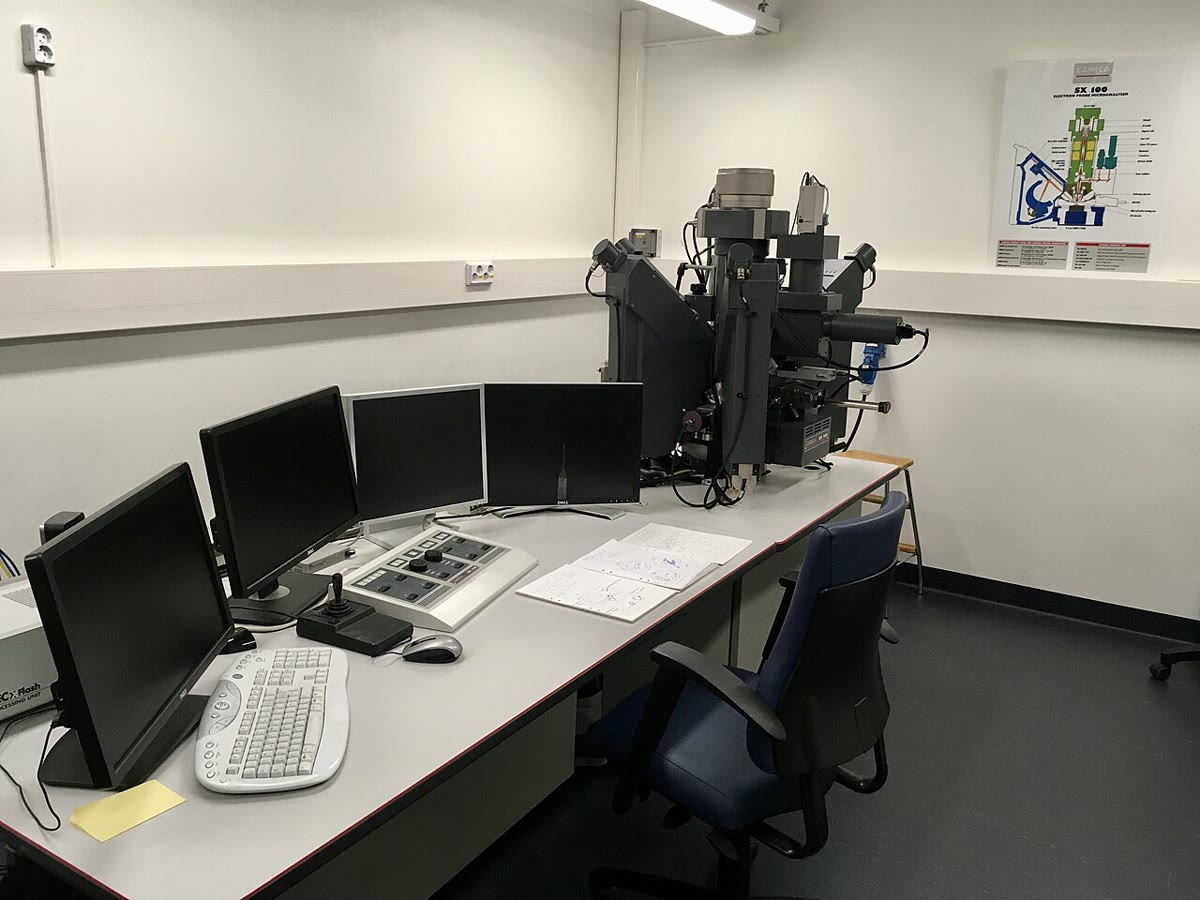
\includegraphics[width=\linewidth]{images/book4/b2-31-microprobe.jpg}
\par\smallskip{\scriptsize Uma \omterm{def:b2:field-lab-methods-2:epma}{microssonda eletrônica}: a coluna eletrônica, com seus espectrômetros
em volta, e a mesa do operador. Fotografia de Kallerna, CC BY-SA 4.0 (Wikimedia Commons).}
\end{minipage}
\end{inthelab}
% ledger: sercE:epma-spot, sercE:coating, photo:b2-31-microprobe

\section{A análise isotópica}\label{sec:b2:field-lab-methods-2:isotopes}

Os \omterm{def:b2:isotope-geochemistry:tracer}{traçadores isotópicos radiogênicos} e as idades (\cref{ch:b2:isotope-geochemistry}) apoiam-se em razões medidas
com 0.01--\qty{0.001}{\percent}, de elementos separados da rocha por dissolução
e cromatografia de troca iônica num laboratório limpo, com ar filtrado (tipicamente da classe 100 a
1000), para que a poeira nada acrescente às pequenas quantidades analisadas.
% ledger: sercT:tims

\begin{definition}[Espectrometria de massa por ionização térmica, ICP-MS multicoletor, viés de massa]\label{def:b2:field-lab-methods-2:tims}
Na \emph{espectrometria de massa por ionização térmica}\index{espectrometria de massa por ionização térmica} (TIMS), um
elemento purificado é depositado num fino filamento metálico e ionizado por aquecimento sob vácuo; os íons
são acelerados por uma diferença de potencial de até \qty{10}{kV}, separados por massa num setor magnético
e coletados. No \emph{ICP-MS multicoletor}\index{ICP-MS multicoletor} os íons vêm de um
plasma indutivamente acoplado, que ioniza elementos difíceis de ionizar termicamente, e vários
coletores medem ao mesmo tempo os feixes de massas diferentes. O \emph{viés de
massa}\index{viés de massa} de uma medida é o desvio de uma razão isotópica medida em relação à razão
verdadeira da amostra causado pelo instrumento, que transmite ou ioniza uma massa mais facilmente que
outra.
\end{definition}
% ledger: sercT:tims, sercM:mcicpms

Os dois instrumentos atingem essa precisão. A TIMS ioniza em geral menos de
\qty{1}{\percent} dos átomos, e seu \omterm{def:b2:field-lab-methods-2:tims}{viés de massa} muda continuamente durante uma corrida. O viés é corrigido fixando a razão de dois isótopos que nenhum
decaimento altera, o que exige um elemento com pelo menos três isótopos, dois deles estáveis e não
radiogênicos. Para o estrôncio, $^{86}\mathrm{Sr}/^{88}\mathrm{Sr}$ é fixada em 0.1194, e uma forma
comum da correção é a lei exponencial.
% ledger: sercT:tims, sercM:mcicpms, cheong14:mass-bias, ciaaw:sr-isotopes

\begin{proposition}[Lei exponencial do viés de massa]\label{prop:b2:field-lab-methods-2:bias}
Suponha-se que toda razão medida entre dois isótopos de massas $m_i$ e $m_j$ se relacione com a razão verdadeira
por $R_{ij}^{\mathrm{true}} = R_{ij}^{\mathrm{meas}}\,(m_i/m_j)^{\beta}$, com um só expoente
$\beta$ para toda a corrida. Então a razão medida $r$ de um par de referência, cujo valor verdadeiro
$r_0$ é conhecido, dá
\begin{equation}
\beta = \frac{\ln(r_0/r)}{\ln(m_k/m_l)}
\label{eq:b2:field-lab-methods-2:beta}
\end{equation}
para o par de referência $k/l$, e toda outra razão é corrigida com o mesmo $\beta$.
\end{proposition}

\begin{proof}
Aplicada ao par de referência, a lei diz $r_0 = r\,(m_k/m_l)^\beta$; tomando logaritmos,
$\ln(r_0/r) = \beta\ln(m_k/m_l)$, que é \eqref{eq:b2:field-lab-methods-2:beta}. O expoente é
comum a todas as razões da corrida por hipótese, de modo que corrige cada uma delas.
\end{proof}

Para o estrôncio o par de referência é $^{86}\mathrm{Sr}/^{88}\mathrm{Sr}$ com $r_0 = 0.1194$, e
a razão $^{87}\mathrm{Sr}/^{86}\mathrm{Sr}$ corrigida é a razão medida vezes
$(m_{87}/m_{86})^\beta$. As abundâncias da CIAAW, \qty{9.86}{\percent} de estrôncio-86 e
\qty{82.58}{\percent} de estrôncio-88, dão o mesmo valor. Cada sessão também analisa um \omterm{def:b2:isotope-geochemistry:standards}{padrão
isotópico de referência}: um laboratório mediu $^{87}\mathrm{Sr}/^{86}\mathrm{Sr} = 0.710252 \pm
0.000007$ no material de referência NBS~987 em sete corridas.
% ledger: cheong14:mass-bias, ciaaw:sr-isotopes

As razões sozinhas não dão uma concentração. Para isso, uma quantidade conhecida de um \emph{traçador isotópico}, uma solução do
elemento artificialmente enriquecida num isótopo, é misturada à amostra dissolvida antes da
química, e a razão é medida na mistura. Os laboratórios de TIMS usam-no tanto para as
concentrações quanto para as razões pai--filho.
% ledger: sercT:tims

\begin{proposition}[Diluição isotópica]\label{prop:b2:field-lab-methods-2:id}
Suponha-se que uma amostra contenha $N_x$ mols de um isótopo de referência $b$ e um traçador $N_s$ mols dele, e sejam
$R_x$, $R_s$ e $R_m$ as razões de um segundo isótopo $a$ para $b$ na amostra, no traçador e
na mistura. Então
\begin{equation}
N_x = N_s\,\frac{R_s - R_m}{R_m - R_x} .
\label{eq:b2:field-lab-methods-2:id}
\end{equation}
Um erro relativo $\varepsilon$ sobre $R_m$ dá a $N_x$ o erro relativo $\mathcal{M}\varepsilon$,
com a amplificação do erro
\begin{equation}
\mathcal{M} = \frac{R_m\,(R_s - R_x)}{(R_s - R_m)(R_m - R_x)} ,
\label{eq:b2:field-lab-methods-2:mag}
\end{equation}
que é mínima quando $R_m = \sqrt{R_s R_x}$.
\end{proposition}
\index{diluição isotópica}

\begin{proof}
O isótopo $a$ conserva-se na mistura: $R_m(N_x + N_s) = R_x N_x + R_s N_s$, de modo que $N_x(R_m - R_x) =
N_s(R_s - R_m)$, que é \eqref{eq:b2:field-lab-methods-2:id}. Sua derivada logarítmica é
$\mathrm{d}\ln N_x/\mathrm{d}\ln R_m = R_m\,[-1/(R_s - R_m) - 1/(R_m - R_x)] = -\mathcal{M}$, com
$\mathcal{M}$ como em \eqref{eq:b2:field-lab-methods-2:mag}. A menos da constante positiva $R_s - R_x$,
$1/\mathcal{M} = (R_s - R_m)(R_m - R_x)/R_m = R_s + R_x - R_m - R_sR_x/R_m$, cuja derivada
$-1 + R_sR_x/R_m^2$ se anula em $R_m = \sqrt{R_sR_x}$, um máximo de $1/\mathcal{M}$.
\end{proof}

A \omterm{prop:b2:field-lab-methods-2:id}{diluição isotópica} não precisa nem de reta de calibração nem de recuperação completa do elemento ao longo
da química: uma vez misturados traçador e amostra, as perdas afetam ambos igualmente. Um traçador de estrôncio
publicado, por exemplo, contém \qty{99.65}{\percent} de estrôncio-84, com
$^{84}\mathrm{Sr}/^{88}\mathrm{Sr} = 561.4$ e $^{86}\mathrm{Sr}/^{88}\mathrm{Sr} = 0.7661$, com
\qty{15.271}{\micro\gram} de estrôncio por grama de solução. Sua razão 86/88 mostra por que o \omterm{def:b2:field-lab-methods-2:tims}{viés
de massa} de uma mistura com traçador não pode ser corrigido fixando $^{86}\mathrm{Sr}/^{88}\mathrm{Sr}$ em seu
valor natural: o traçador deslocou essa razão.
% ledger: cheong14:spike, cheong14:mass-bias

\section{Uma campanha de mapeamento na janela erosiva de Varden}\label{sec:b2:field-lab-methods-2:campaign}

No núcleo do anticlinal de Varden, a erosão cortou a cobertura arenítica e expôs o
embasamento: xisto intrudido por um granito. Uma campanha destinada a abastecer o laboratório começa no
campo. Dois perfis são percorridos de oeste para leste através da janela erosiva, com uma estação a cada
\qty{100}{m}; em cada uma a unidade é registrada, e amostras frescas são coletadas onde a rocha não está
intemperizada, numeradas com a estação e, onde tramas devem ser medidas, orientadas. A figura
mostra o que as estações encontram: das 30, dez estão sobre o granito, dez sobre a cobertura arenítica, uma sobre
o xisto, uma sobre o calcário e oito sobre o aluvião do fundo do vale, onde nenhuma rocha
aflora.

\begin{omfigure}
\centering
\begin{tikzpicture}
\begin{axis}[axis equal image, xmin=2.4, xmax=4.6, ymin=3.1, ymax=5.0, width=0.66\linewidth,
  tick label style={font=\scriptsize}, xlabel={leste (km)}, ylabel={norte (km)},
  label style={font=\small}]
% units: figdata/shared/region.py (read only); stations: figdata/bachelor-2/labmethods.py part stations
\addplot[lith schist, draw=black, line width=0.3pt, even odd rule] table {figdata/out/shared-region-unit-schist.dat};
\addplot[lith granite, draw=black, line width=0.3pt, even odd rule] table {figdata/out/shared-region-unit-granite.dat};
\addplot[om lith={icsTriassic!35}{om sand}, draw=black, line width=0.3pt, even odd rule] table {figdata/out/shared-region-unit-sandstone.dat};
\addplot[om lith={icsJurassic!40}{om limestone}, draw=black, line width=0.3pt, even odd rule] table {figdata/out/shared-region-unit-limestone.dat};
\addplot[om lith={icsJurassic!15}{om shale}, draw=black, line width=0.3pt, even odd rule] table {figdata/out/shared-region-unit-shale.dat};
\addplot[lith alluvium, draw=black, line width=0.3pt, even odd rule] table {figdata/out/shared-region-unit-alluvium.dat};
\addplot[river] table {figdata/out/shared-region-river.dat};
\addplot[only marks, mark=*, mark size=1.6pt, mark options={fill=white, draw=black}]
  table[x=x_km, y=y_km] {figdata/out/bachelor-2-labmethods-stations.dat};
\addplot[only marks, mark=*, mark size=1.6pt, mark options={fill=omThm, draw=black},
  x filter/.expression={\thisrow{unit}==2 ? x : nan}]
  table[x=x_km, y=y_km] {figdata/out/bachelor-2-labmethods-stations.dat};
\node[font=\scriptsize, fill=white, inner sep=1pt, anchor=east] at (axis cs:2.76,3.7) {1};
\node[font=\scriptsize, fill=white, inner sep=1pt, anchor=west] at (axis cs:4.24,3.7) {15};
\node[font=\scriptsize, fill=white, inner sep=1pt, anchor=east] at (axis cs:2.76,4.4) {16};
\node[font=\scriptsize, fill=white, inner sep=1pt, anchor=west] at (axis cs:4.24,4.4) {30};
\draw[black, line width=0.5pt] (axis cs:3.5,4.44) -- (axis cs:3.5,4.62);
\node[font=\scriptsize, fill=white, inner sep=1pt, anchor=south] at (axis cs:3.5,4.62) {estação 23};
\pic at (axis cs:4.45,4.75) {northarrow};
\end{axis}
\end{tikzpicture}
\par\smallskip{\small A janela de embasamento das Varden Hills com as 30 estações de dois perfis
oeste--leste, a \qty{100}{m} um do outro. Pontos vermelhos: estações sobre o granito. Rosa com cruzes: granito; cinza: xisto; roxo: arenito
triássico; azul: calcário jurássico; azul-claro: folhelho jurássico; creme: aluvião do rio, que
corre para leste. A
amostra de granito do problema de fim de semana vem da estação 23.}
\end{omfigure}

\begin{inthefield}[Amostrar para o laboratório]
\centering
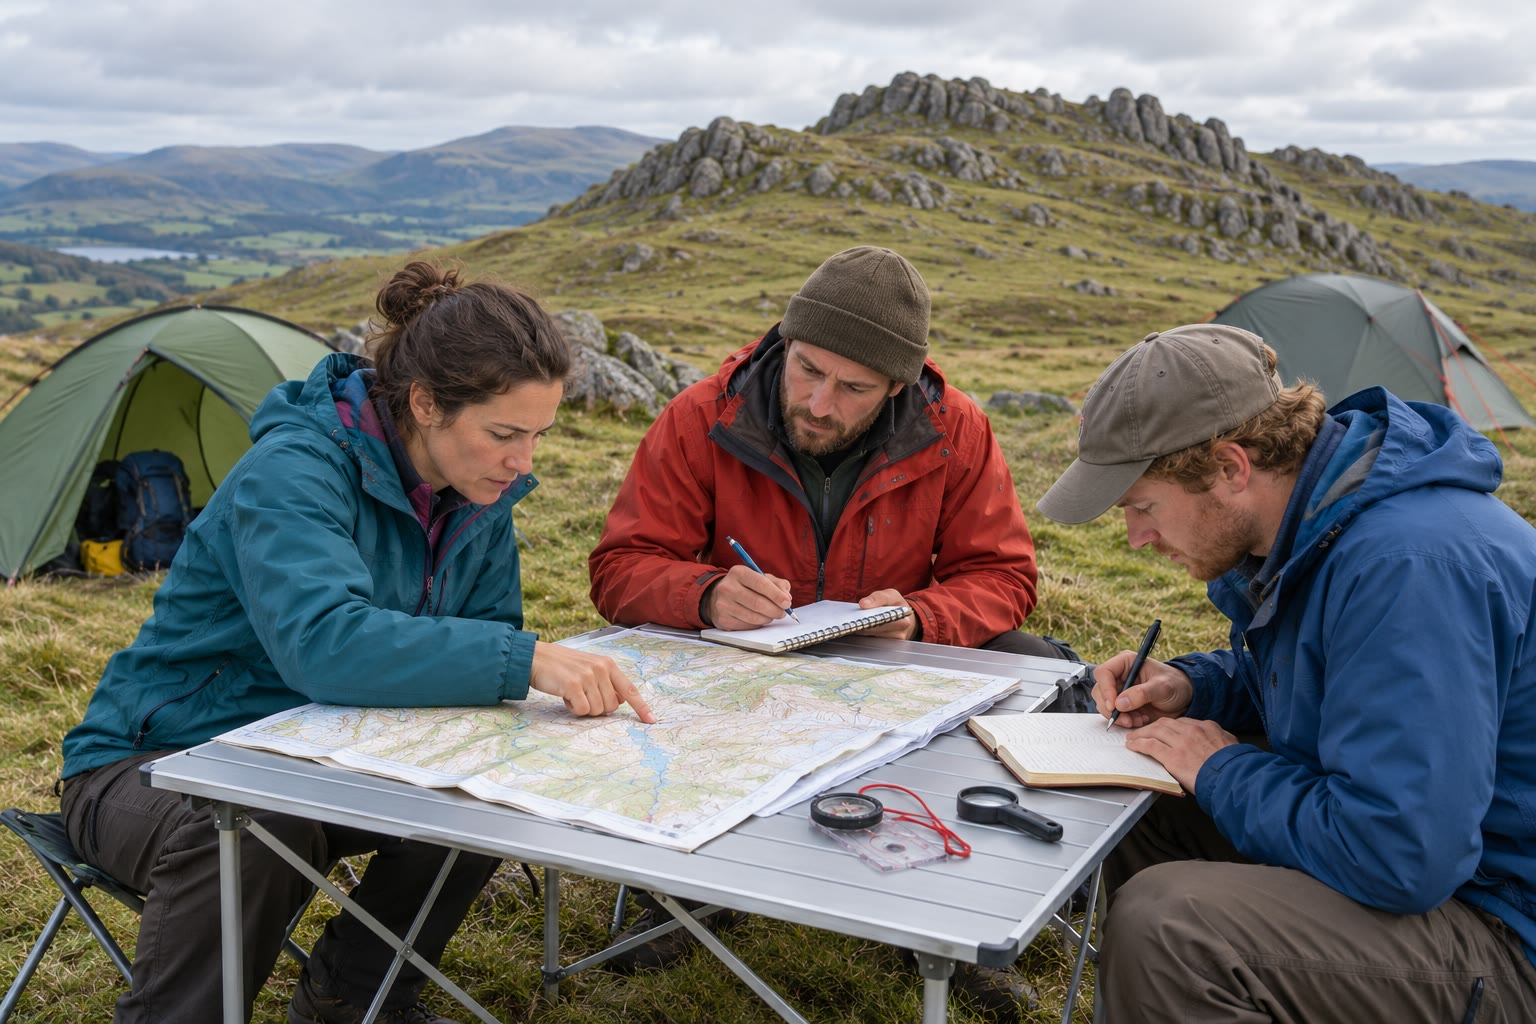
\includegraphics[width=0.56\linewidth]{images/book4/ai/b2-field-camp.jpg}
\par\smallskip{\small Uma equipe de campo planeja os perfis do dia seguinte (ilustração gerada por IA).}
\par\medskip\raggedright
À noite a equipe passa as estações para o mapa, verifica se cada número de amostra das
cadernetas corresponde a um saco, e decide que amostras vão para que laboratório. Uma amostra de cada unidade
vai para o laboratório de laminação; o granito e o xisto mais frescos vão
para britagem e análise de rocha total; algumas amostras de granito são reservadas para os isótopos. O
número da estação acompanha cada amostra em todas as etapas, do saco à lâmina delgada, ao
pó, à pastilha e à linha de uma tabela de dados, de modo que qualquer resultado estranho possa ser rastreado até seu
afloramento.
\end{inthefield}

\section{A qualidade de um número}\label{sec:b2:field-lab-methods-2:quality}

Cada etapa da cadeia acrescenta seu próprio erro, e os métodos deste capítulo mostram os dois tipos que
os livros de química distinguem. A \omterm{def:b2:field-lab-methods-2:modal}{contagem de pontos} e as razões isotópicas têm erros sobretudo aleatórios, que
diminuem à medida que as contagens crescem, como $1/\sqrt n$; a calibração tem erros sistemáticos, que a repetição não
reduz e que só um material de referência revela. A figura das análises de sílica mostra
ambos: as barras são a precisão do método, e um ponto que se afasta de zero muitas vezes sua barra
dividida pela raiz quadrada do número de análises é um viés. O mesmo elemento medido por dois
métodos, o estrôncio por FRX e por \omterm{prop:b2:field-lab-methods-2:id}{diluição isotópica}, é uma verificação adicional, pois os dois não compartilham
calibração. Os resultados são relatados com sua incerteza, arredondados a ela, e com os materiais de
referência analisados junto; um número sem eles não pode ser comparado com nenhum outro.

\section*{Exercícios}\label{sec:b2:field-lab-methods-2:exercises}

Dados para os exercícios, salvo indicação em contrário: massas atômicas H 1.008, O 15.999, Mg 24.305, Al
26.982, Si 28.085, K 39.098, Sr 87.62; massas isotópicas $^{86}\mathrm{Sr}$ 85.909261,
$^{87}\mathrm{Sr}$ 86.908878, $^{88}\mathrm{Sr}$ 87.905612; estrôncio natural
$^{84}\mathrm{Sr}/^{86}\mathrm{Sr} = 0.05680$, \qty{9.86}{\percent} de $^{86}\mathrm{Sr}$; o traçador
do texto, $^{84}\mathrm{Sr}/^{86}\mathrm{Sr} = 732.8$, \qty{0.13599}{\percent} de
$^{86}\mathrm{Sr}$, massa atômica 83.9242, \qty{15.271}{\micro\gram\per\gram}. Arredonde a três
algarismos significativos salvo indicação em contrário.
% ledger: ciaaw:H, ciaaw:O, ciaaw:Mg, ciaaw:Al, ciaaw:Si, ciaaw:K, ciaaw:sr-isotopes, cheong14:spike

\begin{exercise}[$\star$]\label{exo:b2:field-lab-methods-2:1}
(a) Dê nome à textura ou ao cristal: (i) um diabásio no qual ripas de plagioclásio estão inteiramente englobadas em
grandes cristais de augita; (ii) um mármore de grãos de calcita de tamanho igual cujos limites retos se encontram
três a três; (iii) um cristal de estaurolita de \qty{5}{mm} de comprimento repleto de inclusões de quartzo num mica xisto;
(iv) uma granada envolvida por uma orla contínua de plagioclásio e piroxênio. (b) Três limites de grão
se encontram a \ang{104}, \ang{128} e \ang{128}. Encontre a razão entre a tensão do limite oposto
ao ângulo de \ang{104} e a dos outros.
\end{exercise}

\begin{exercise}[$\star$]\label{exo:b2:field-lab-methods-2:2}
Uma rocha de granulação grossa contém \qty{25}{\percent} de quartzo, 15 de feldspato alcalino, 40 de plagioclásio, 12 de
biotita e 8 de hornblenda. (a) Recalcule Q, A e P. (b) Encontre P/(A+P) e dê nome à rocha. (c) Encontre
seu índice de cor e qualifique-o.
\end{exercise}

\begin{exercise}[$\star$]\label{exo:b2:field-lab-methods-2:3}
Uma contagem de 800 pontos encontra um mineral a \qty{12}{\percent}. (a) Encontre o desvio-padrão dessa
proporção, e seu valor relativo. (b) Qual seria ele com 3200 pontos?
\end{exercise}

\begin{exercise}[$\star$]\label{exo:b2:field-lab-methods-2:4}
Um pó de \qty{0.8000}{g} pesa \qty{0.7712}{g} após a calcinação, e o resíduo é fundido com
\qty{8.0000}{g} de fundente. (a) Encontre a \omterm{def:b2:field-lab-methods-2:xrf}{perda ao fogo}. (b) Encontre a fração mássica da amostra na
pastilha. (c) O vidro contém \qty{5.20}{\percent} de \ce{SiO2}. Encontre a sílica do pó calcinado
e do pó original.
\end{exercise}

\begin{exercise}[$\star\star$]\label{exo:b2:field-lab-methods-2:5}
(a) Quantos pontos são necessários para medir um mineral acessório que constitui \qty{2}{\percent} de uma rocha
com um erro-padrão relativo de \qty{10}{\percent}? (b) E um mineral que constitui \qty{30}{\percent},
com o mesmo erro relativo? (c) Comente o esforço que um mineral raro exige.
\end{exercise}

\begin{exercise}[$\star\star$]\label{exo:b2:field-lab-methods-2:6}
Nos resultados do USGS da figura, o riolito RGM-1 deu \ce{SiO2} $= 72.89$ com desvio-padrão
de 0.19 em 20 análises (recomendado 73.45), e o basalto BCR-2 deu 54.17 com 0.13 em
20 análises (recomendado 54.1). (a) Encontre a recuperação de cada um, em porcentagem. (b) Encontre o desvio-padrão
de cada média, e exprima cada diferença em relação ao valor recomendado em unidades dele.
(c) Que resultado mostra um viés? O método é menos preciso para o RGM-1?
\end{exercise}

\begin{exercise}[$\star\star$]\label{exo:b2:field-lab-methods-2:7}
Uma análise de microssonda de uma flogopita pura, $\mathrm{KMg_3AlSi_3O_{10}(OH)_2}$, deve ser verificada.
(a) Encontre a massa molar da fórmula e a fração mássica de \ce{H2O} que ela contém. (b) Encontre as
frações mássicas de \ce{K2O}, \ce{MgO}, \ce{Al2O3} e \ce{SiO2}, e o total que uma análise exata
daria. (c) Por que um total de cerca de \qty{96}{\percent} para uma mica não é uma análise ruim?
\end{exercise}

\begin{exercise}[$\star\star$]\label{exo:b2:field-lab-methods-2:8}
Uma corrida de TIMS num padrão de estrôncio dá $^{86}\mathrm{Sr}/^{88}\mathrm{Sr} = 0.11905$ e
$^{87}\mathrm{Sr}/^{86}\mathrm{Sr} = 0.71062$. (a) Encontre o expoente $\beta$ da lei exponencial.
(b) Corrija a razão $^{87}\mathrm{Sr}/^{86}\mathrm{Sr}$, com cinco casas decimais. (c) O isótopo leve ou
o pesado foi favorecido na corrida?
\end{exercise}

\begin{exercise}[$\star\star$]\label{exo:b2:field-lab-methods-2:9}
Para verificar sua \omterm{prop:b2:field-lab-methods-2:id}{diluição isotópica}, um laboratório adiciona a \qty{0.0500}{g} do basalto de referência BHVO-2
\qty{0.1000}{g} do traçador do texto, e mede $^{84}\mathrm{Sr}/^{86}\mathrm{Sr} =
0.874$ na mistura. (a) Encontre os mols de $^{86}\mathrm{Sr}$ na alíquota de traçador. (b) Encontre os
mols de $^{86}\mathrm{Sr}$ na amostra, e sua concentração de estrôncio em ppm. (c) Compare com
os \qty{394.1}{ppm} recomendados.
\end{exercise}

\begin{exercise}[$\star\star\star$]\label{exo:b2:field-lab-methods-2:10}
Para o traçador de estrôncio do texto ($R_s = 732.8$, $R_x = 0.05680$): (a) encontre a razão da mistura
que minimiza a amplificação do erro, e seu valor ali; (b) calcule $\mathcal M$ para
$R_m = 0.1$, 0.5, 1.664 e 100; (c) explique por que uma mistura próxima de um dos dois membros extremos deve ser
evitada, e quanta liberdade o analista tem na prática.
\end{exercise}

\begin{exercise}[$\star\star\star$]\label{exo:b2:field-lab-methods-2:11}
Uma contagem num granito encontra 400 pontos de feldspato, \qty{62}{\percent} deles de plagioclásio. (a) Tratando o
plagioclásio entre os pontos de feldspato como uma contagem binomial, encontre o desvio-padrão de
P/(A+P). (b) A quantos desvios-padrão o resultado está do limite do granodiorito? (c) Quantos
pontos de feldspato o colocariam a dois desvios-padrão do limite?
\end{exercise}

\begin{exercise}[$\star\star\star$]\label{exo:b2:field-lab-methods-2:12}
Um mineral ocupa uma fração $p$ de uma rocha. (a) Mostre que a probabilidade de que $n$ pontos independentes
o errem todos é $(1-p)^n$. (b) Quantos pontos dão pelo menos \qty{95}{\percent} de chance de
atingir ao menos uma vez um mineral que constitui \qty{1}{\percent} da rocha? (c) O mesmo para o zircão a
\qty{0.05}{\percent}, e conclua sobre como um mineral acessório deve ser procurado.
\end{exercise}

\section*{Problema de fim de semana}

\begin{problem}[{Problema de fim de semana --- do afloramento à análise}]\label{pb:b2:field-lab-methods-2:1}
% invented sample; data: ledger rows below; values: calc/ch31.py
A amostra VH-23 do granito de Varden foi coletada na estação 23 da campanha. Uma lâmina delgada teve
seus pontos contados numa malha regular de 1200 pontos: quartzo 372, feldspato alcalino 348, plagioclásio 324,
biotita 108, muscovita 36, óxidos opacos 12. Um pó de \qty{0.8000}{g} pesou \qty{0.7949}{g}
após calcinação a \qty{925}{\celsius} e foi fundido com \qty{8.0000}{g} de fundente. Pastilhas de três
materiais de referência deram estas intensidades de \ce{SiO2} (milhares de contagens por segundo, kcps): BCR-2,
recomendado \qty{54.1}{\percent}, 21.66; AGV-2, 59.3, 23.70; RGM-1, 73.45, 29.37; a pastilha do granito
deu 28.63. Os outros óxidos do granito somam \qty{27.15}{\percent}. Para os isótopos,
\qty{0.1000}{g} de pó foi dissolvido e misturado com \qty{0.2500}{g} do traçador do texto;
supõe-se que a amostra tem as abundâncias naturais de estrôncio dos exercícios. Use os dados dos
exercícios.

\noindent\textbf{Parte I --- A moda.}
\begin{enumerate}
  \item Encontre a proporção modal de cada mineral.
  \item Encontre o desvio-padrão da proporção de quartzo, e o desvio-padrão relativo
        da proporção de muscovita.
  \item Encontre $M$ e o índice de cor $M'$, e qualifique a rocha.
  \item Recalcule Q, A e P a uma soma de 100.
  \item Encontre P/(A+P) e dê nome à rocha no \omterm{def:b2:magmatic-series:qapf}{diagrama QAPF}.
  \item Com o desvio-padrão binomial de P/(A+P) sobre os 672 pontos de feldspato, o nome
        é seguro?
  \item Quantos pontos levariam o desvio-padrão da proporção de quartzo a um
        ponto percentual?
\end{enumerate}

\noindent\textbf{Parte II --- A sílica por fluorescência de raios X.}
\begin{enumerate}[resume]
  \item Encontre a \omterm{def:b2:field-lab-methods-2:xrf}{perda ao fogo}.
  \item Encontre a fração mássica da amostra na pastilha, e a sílica do vidro se o
        pó calcinado contém \qty{72}{\percent}.
  \item Ajuste a reta de mínimos quadrados $c = aI + b$ pelos três materiais de referência; dê $a$ com
        quatro casas decimais e $b$ com duas.
  \item Encontre o \ce{SiO2} do granito, com duas casas decimais.
  \item Encontre os resíduos dos três materiais de referência. A reta é adequada?
  \item Some os óxidos e a \omterm{def:b2:field-lab-methods-2:xrf}{perda ao fogo}. O procedimento do USGS repetiria essa análise?
  \item Recalcule a sílica a uma soma de 100 sem os voláteis.
\end{enumerate}

\noindent\textbf{Parte III --- O viés de massa.}
\begin{enumerate}[resume]
  \item A partir das abundâncias da CIAAW, encontre a razão natural $^{86}\mathrm{Sr}/^{88}\mathrm{Sr}$ e compare-a
        com o valor usado para normalizar.
  \item Uma alíquota sem traçador dá $^{86}\mathrm{Sr}/^{88}\mathrm{Sr} = 0.11853$. Encontre $\beta$ com
        quatro casas decimais.
  \item Ela dá $^{87}\mathrm{Sr}/^{86}\mathrm{Sr} = 0.71655$. Corrija-a, com cinco casas decimais.
  \item Encontre o viés por unidade de massa, em porcentagem.
  \item Por que essa correção não pode ser feita na mistura com traçador da Parte IV?
\end{enumerate}

\noindent\textbf{Parte IV --- A diluição isotópica.}
\begin{enumerate}[resume]
  \item Verifique que o traçador contém \qty{99.65}{\percent} de estrôncio-84 e \qty{0.13599}{\percent}
        de estrôncio-86.
  \item Encontre os mols de estrôncio e de $^{86}\mathrm{Sr}$ na alíquota de traçador, com quatro
        algarismos significativos.
  \item Verifique os valores $R_s = 732.8$ e $R_x = 0.05680$ dos exercícios.
  \item A razão corrigida da mistura é $R_m = 1.6812$. Encontre os mols de $^{86}\mathrm{Sr}$
        da amostra.
  \item Encontre a amplificação do erro. Com $R_m$ conhecida a \qty{0.01}{\percent} e a concentração
        do traçador a $\pm\qty{0.031}{\micro\gram\per\gram}$, encontre a incerteza relativa
        do resultado.
  \item Encontre a concentração de estrôncio do granito de Varden, em ppm.
\end{enumerate}
\end{problem}
% ledger: bgsI:qapf, bgsI:colour-index, usgsT:procedure, usgsT:sio2-table, ciaaw:sr-isotopes, cheong14:spike, cheong14:mass-bias
